\documentclass{article}

% if you need to pass options to natbib, use, e.g.:
%     \PassOptionsToPackage{numbers, compress}{natbib}
% before loading neurips_2024


% ready for submission
\usepackage{neurips_2024}
\usepackage{natbib}

\usepackage{graphicx}
\usepackage[utf8]{inputenc} % allow utf-8 input
\usepackage[T1]{fontenc}    % use 8-bit T1 fonts
\usepackage{hyperref}       % hyperlinks
\usepackage{url}            % simple URL typesetting
\usepackage{booktabs}       % professional-quality tables
\usepackage{amsfonts}       % blackboard math symbols
\usepackage{nicefrac}       % compact symbols for 1/2, etc.
\usepackage{microtype}      % microtypography
\usepackage{xcolor}         % colors


\title{Escherichia Coli Ceftriaxone Resistance}

% The \author macro works with any number of authors. There are two commands
% used to separate the names and addresses of multiple authors: \And and \AND.
%
% Using \And between authors leaves it to LaTeX to determine where to break the
% lines. Using \AND forces a line break at that point. So, if LaTeX puts 3 of 4
% authors names on the first line, and the last on the second line, try using
% \AND instead of \And before the third author name.

\author{%
  D. Bugatti, N. Dupertuis, A. Giacomuzzi, N. Oberholzer\\
  Foundations of Data Science\\
  Department of Health Science and Technology\\
  ETH Zürich\\
}



\begin{document}
\maketitle

\begin{abstract}
Antibiotic resistance is a growing global health threat, requiring fast and accurate diagnostic tools to guide treatment decisions. In this project, we examine the resistance of Escherichia coli to Ceftriaxone using MALDI-TOF mass spectrometry data from the DRIAMS dataset. The dataset contains 1368 clinical samples with 5999 spectral features. We apply and compare four machine learning models: Support Vector Machine (SVM), Logistic Regression, Random Forest, and k-Nearest Neighbors (kNN). Feature selection and class imbalance handling are used to improve predictive performance. Logistic Regression achieved the highest overall accuracy and ROC AUC, while Random Forest showed perfect recall, illustrating trade-offs between sensitivity and specificity. These results highlight the potential of MALDI-TOF spectral data for predicting antibiotic resistance in E. coli and demonstrate how machine learning can support rapid diagnostics. The study also points to key deployment considerations, such as model robustness and interpretability, that are critical for real-world clinical applications.
\end{abstract}


\section{Introduction}

Antibiotic resistance is a rapidly escalating global health threat, significantly complicating the treatment of bacterial infections and leading to higher mortality, morbidity, and healthcare costs worldwide. Recent data underscore the severity of this issue; for example, a systematic review conducted by \citet{IranBacteria} revealed that 87.5\% of bacterial isolates obtained from clinical specimens in Northern Iran showed resistance to at least one commonly prescribed antibiotic. Given ongoing selective pressure, this alarming prevalence is likely even higher today, emphasizing the critical need for effective diagnostic tools to rapidly identify resistant strains and guide therapeutic decisions.
Matrix-Assisted Laser Desorption/Ionization Time-of-Flight (MALDI-TOF) mass spectrometry has emerged as a powerful technique for rapid microbial identification and characterization. A recent large-scale study compiled MALDI-TOF mass spectra from over 300,000 bacterial and fungal samples and successfully applied machine learning techniques to predict antimicrobial resistance phenotypes directly from these spectra \citep{datasetExplaination, Astudillo2024}. Leveraging such techniques could significantly reduce the time required for identifying resistance profiles compared to traditional phenotypic testing methods.
In this project, we specifically focus on evaluating the predictive capabilities of classical machine learning models - Support Vector Machine (SVM), Logistic Regression, Random Forest, and k-Nearest Neighbors (kNN) - for detecting Ceftriaxone resistance in \textit{Escherichia coli} using MALDI-TOF spectra DRIAMS dataset. Our primary aim is to assess the real-world applicability and performance of these machine learning algorithms in accurately distinguishing Ceftriaxone-resistant strains from sensitive ones.

The scientific hypothesis tested in this study is that classical machine learning algorithms, trained on MALDI-TOF spectral data, can achieve clinically relevant performance (ROC AUC > 0.85) in predicting Ceftriaxone resistance in \textit{Escherichia coli}.

\section{Methods}

\subsection{Data Source}
The dataset used in this study was obtained from the publicly available DRIAMS database, which contains MALDI-TOF mass spectrometry data collected from clinical bacterial and fungal isolates \citep{datasetExplaination}. Specifically, we focused on 1368 clinical isolates of \textit{Escherichia coli}, tested for resistance against Ceftriaxone.

\subsection{Data Preprocessing}
The dataset initially contained 5999 spectral features (normalized intensities between 0 and 1), an integer label (1 for resistant, 0 for sensitive), and a metadata column labeled "Unnamed: 0" identifying the MALDI-TOF instrument used (“MALDI\_1” or “MALDI\_2”). To prevent potential model bias or overfitting based on instrumentation differences, the metadata column was removed. Data was further checked for missing values and duplicate entries; neither were found.

\subsection{Feature Selection}
As the dataset contains more features than samples (5999 features vs. 1368 samples), a feature
selection needed to be performed before fitting with either a filter, wrapper or embedded method. To ensure
that some features can be removed without losing too much information, we created a Pearson’s correlation matrix of the features and plotted its heatmap (Figure \ref{fig:Heatmap of Pearson's correlation matrix}) with matplotlib \citep{matplotlib} and seaborn \citep{seaborn}.\\

\begin{figure}
	\centering
	\includegraphics[width=0.9\textwidth]{heatmap.png}
	 \vspace{-3em}
	\caption{Heatmap of Pearson's Correlation Matrix}
    \label{fig:Heatmap of Pearson's correlation matrix}
\end{figure}

Except the trivial white line that divides the heatmap in half, there are numerous white and dark blue spots, which indicate high positive or negative correlation. Thanks to the graph we can safely assume that most of the variable are correlated, and therefore a filter will not only diminish the probability of overfitting (as mentioned earlier, a higher number of features than samples must always be avoided), but also focus the attention of the model onto non-collinear and highly explanatory features. 

\subsection{Class Imbalance Handling}
Another issue that must be addressed is the class imbalance; 81.5\% of the bacteria samples are resistant to Ceftriaxone, and only 18.5\% are not. There are several ways to help the model focus more onto the minority class. One solution is undersampling the majority class, but we ruled this out, because our dataset already has a relatively low number of samples. Another solution is oversampling the minority, but we rejected it because the duplicated samples would have identical values, therefore increasing the chance of overfitting which is already a concern with this dataset. The solution we chose as best is balancing the class weight in the model. This method doesn't involve dataset alterations, it instead adjusts the training process by giving more importance to mistakes made on the minority class. Specifically, by multiplying such errors by a weight, usually set inversely proportional to the minority class frequency.

\subsection{Dataset Split}

The dataset has been split into training and testing sets with an 85\% ratio for training and a 15\% ratio for testing. This leaves 208 samples for testing and 1178 samples for training.

\subsection{Machine Learning Models}

We evaluated four classical machine learning models, each briefly described and tuned explicitly using grid search with 5-fold cross-validation to optimize predictive performance:

\subsubsection{Support Vector Machine (SVM)}
Support Vector Machine (SVM) makes its prediction based on hyperplane divisions on the multidimensional feature space. It is therefore extremely important for the success of the model, to select only the highly explanatory features. 

We created a flowchart (Figure \ref{fig:Flowchart of the implemented SVM Model}) which should help visualize the model.

\begin{figure}[h]
	\centering
	\includegraphics[width=1.0\textwidth]{FlowChart.png}
	 \vspace{0em}
	\caption{Flowchart of the implemented SVM Model}
    \label{fig:Flowchart of the implemented SVM Model}
    
\end{figure}

As SVM is so dependent on the selected features, we decided to implement a wrapper method which unifies feature selection and SVM model tuning into a grid search cross validation environment to iterate the method for every combination of hyperparameters possible for both feature selection and SVM. At first, a number K of features are selected to train the SVM. The non selected features are discarded. The selection algorithm we deemed best is ANOVA, because it selects the features whose variance contributes the most to the variance in the label. Since SVMs require highly explanatory features, this selection method aligns perfectly with their requirements. After the filtering process, a Support Vector Machine (SVM) model is fitted with a combination of two hyperparameters: C, which represents the strength of the penalty applied through L2 regularization, and Kernel, which determines the shape of the division between classes.

Thanks to pipelining, the same grid search cross validation (5 folds) was used to iterate between all of the combinations of the three hyperparameters:
 
\begin{itemize}
  \item Feature selection's K: [500, 1000, 1250, 1500, 1750]
  \item SVM's C: [10, 100, 125, 150, 175]
  \item SVM's Kernel: ["linear", "poly", "rbf", "sigmoid"]
\end{itemize}

The best model was then selected using the average from each fold of the ROC AUC score. 

\hfill\break
\hfill\break


\subsubsection{Random Forest (RF)}
Random Forest (RF) is an ensemble learning algorithm that builds multiple decision trees during training and outputs the class that is the mode of the classes predicted by individual trees. Random Forest was selected for its robustness to noisy and high-dimensional datasets, ease of use, and inherent handling of non-linear relationships without extensive data preprocessing.

To optimize model performance, we performed hyperparameter tuning using grid search with 5-fold cross-validation. The hyperparameters considered were:

\begin{itemize}
    \item \textbf{Number of Trees (\texttt{n\_estimators})}: [300, 350, 400, 450, 500].
    \item \textbf{Maximum Tree Depth (\texttt{max\_depth})}: [None, 10, 20].
    \item \textbf{Minimum Samples for Node Splitting (\texttt{min\_samples\_split})}: [2, 5, 10].
\end{itemize}

To address the significant class imbalance present in the dataset (81.5\% resistant vs. 18.5\% sensitive), the parameter \texttt{class\_weight="balanced"} was set, ensuring increased penalization of misclassification errors for the minority class during training.

Hyperparameter tuning was evaluated using the Receiver Operating Characteristic Area Under the Curve (ROC AUC), specifically selected for its effectiveness in evaluating models trained on imbalanced datasets. This aligns with our aim of achieving clinically relevant predictive performance (ROC AUC > 0.85).

\subsubsection{Logistic Regression}

Within the scope of predictive modeling, we tested logistic regression as a simple and interpretable model for binary classification tasks. Despite its simplicity, it showed solid performance in our experiment: with an accuracy of around 0.8942, it clearly outperformed the baseline random guess level of 50\% for a binary target variable. However, accuracy alone reveals little about the true model quality, so we additionally analyzed the confusion matrix.


\subsubsection{k-Nearest Neighbors (kNN)}
In our data science project, each team member was tasked with training a different machine learning model on the same dataset. My chosen model is K-Nearest Neighbors (KNN).
Before training, we applied a basic data filtering technique to reduce dimensionality and improve relevance. Specifically, we removed all variables with more than 80\% correlation to avoid multicollinearity. We did not treat K as a tunable hyperparameter at this stage, but it's important to note that the choice of K has a strong impact on model performance and should ideally be validated. KNN is a lazy learning algorithm, meaning it doesn’t build a model during training. Instead, when it receives a new data point, it:
\begin{itemize}
    \item Calculates the distance to all points in the training set (e.g., using Euclidean distance).
    \item Selects the K closest neighbors.
    \item Looks at their labels.
    \item Assigns the most common label among those neighbors to the new data point.
\end{itemize}

\subsection{Evaluation Metrics}
Given the highly imbalanced nature of our dataset (81.5\% resistant vs. 18.5\% sensitive samples), standard accuracy alone is insufficient to reliably evaluate predictive performance. To address this, we employed multiple complementary evaluation metrics specifically chosen for their effectiveness in assessing performance on imbalanced data:
\begin{itemize}
    \item \textbf{ROC AUC:} Primary metric assessing model discrimination independently from class thresholds.
    \item \textbf{Precision and Recall:} Measures to interpret false positive/negative trade-offs explicitly.
    \item \textbf{F1-Score:} Harmonic mean balancing precision and recall.
    \item \textbf{Accuracy:} Provided as a reference but interpreted cautiously given class imbalance.
\end{itemize}
These metrics collectively provide a comprehensive evaluation of each model, enabling clear insight into the practical strengths and weaknesses of each approach.

\section{Results}

The following models have been trained and evaluated on the same dataset split, enabling an equal comparison and evaluation of their performance. They have been developed with Scikit-learn's \citep{scikit-learn}, Pandas's \citep{pandas} and numpy's \citep{numpy} algorithms and documentations. 

\subsection{SVM}

The model that performed the best during cross validation was an SVM with rbf kernel and C coefficient equal to 125 fitted on 1500 out of the 5999 total features. After retraining the model on the whole training dataset, we evaluated on the test dataset and obtained the following results:

\begin{figure}[h]
	\centering
	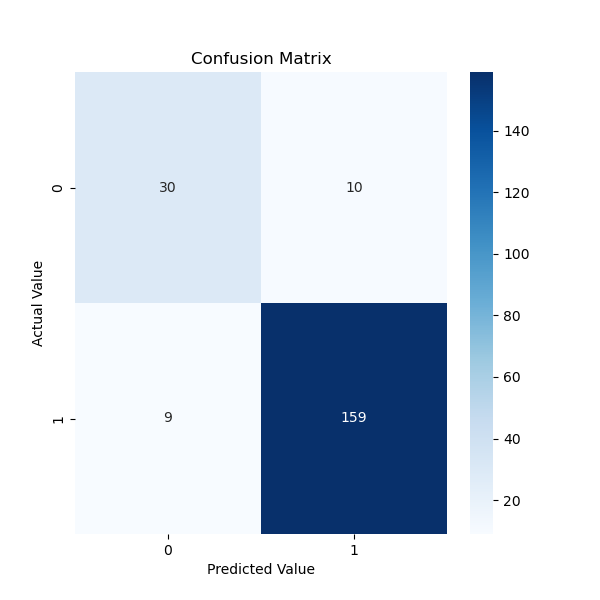
\includegraphics[width=0.6\textwidth]{confusion_matrix_SVM.png}
	 \vspace{-1em}
	\caption{Confusion Matrix for the SVM Model}
    \label{fig:Confusion Matrix of the SVM}
\end{figure}

The statistics calculated from the confusion matrix (Figure \ref{fig:Confusion Matrix of the SVM}) are the following (Table \ref{tab:evaluation_metrics_SVM}): 
\begin{table}[h!]
\centering
\caption{Evaluation Metrics for the SVM Model}
\label{tab:evaluation_metrics_SVM}
\begin{tabular}{|l|c|}
\hline
\textbf{Metric} & \textbf{Value} \\
\hline
Accuracy  & 0.9087 \\
Precision & 0.9408 \\
Recall    & 0.9464 \\
F1 Score  & 0.9436 \\
\hline
\end{tabular}
\end{table}
Accuracy is the lowest of the scores, and this is explained by looking at the confusion matrix. The model is quite good at predicting positive bacteria samples, but performs quite worse in predicting negative samples. As accuracy gives the same importance to both positive and negative samples, it is comprehensibly the lowest score. The calculated ROC AUC score was instead a 0.9149. Overall, the model performed reasonably well, however there still might be space for improvements on the hyperparameters.
Since the filtering process was itself part of the model and caused the model to perform better, it is not only fair, but also right to compare the model with specific feature selection with the other models, which have selected their features in a different way.

\clearpage
\subsection{Random Forest}


The optimal hyperparameter combination found through cross-validation was:
\begin{itemize}
    \item \texttt{n\_estimators} = 500
    \item \texttt{max\_depth} = 20
    \item \texttt{min\_samples\_split} = 5
\end{itemize}

The optimized Random Forest model was retrained on the entire training set (1178 samples) and evaluated on the test set (208 samples). Figure \ref{fig:rf_confusion_matrix} illustrates the confusion matrix for the Random Forest classifier on the test dataset.

\begin{figure}[h]
  \centering
  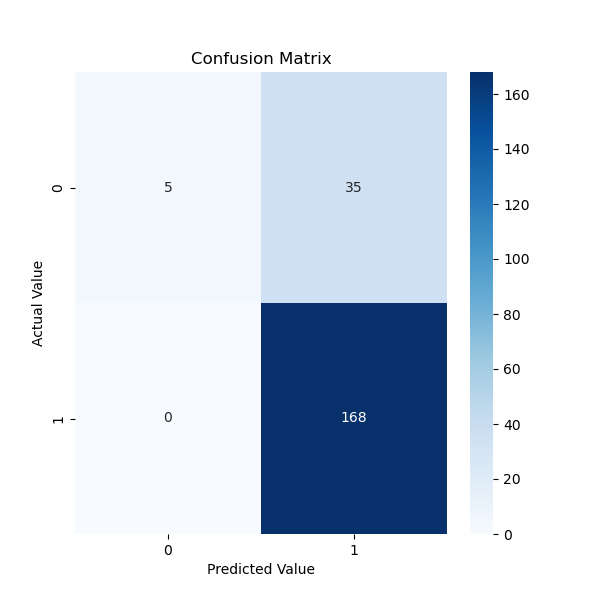
\includegraphics[width=0.6\textwidth]{confusion_matrix_Random_Forest.png}
  \caption{Confusion Matrix for the RF Model}
  \label{fig:rf_confusion_matrix}
\end{figure}

From the confusion matrix, the following performance metrics were calculated:

\begin{table}[h]
\centering
\caption{Evaluation Metrics for the RF Model}
\label{tab:Random Forest Performance Metrics}
\begin{tabular}{|l|c|}
\hline
\textbf{Metric} & \textbf{Value} \\
\hline
ROC AUC   & 0.8242 \\
Accuracy  & 0.8269 \\
Precision & 0.8235 \\
Recall    & 1.0000 \\
F1 Score  & 0.9032 \\
\bottomrule
\end{tabular}
\end{table}

Table \ref{tab:Random Forest Performance Metrics} shows that the Random Forest model demonstrated a perfect recall (1.0); correctly identifying all resistant samples. However, this high recall came at the cost of a lower precision (0.8267), indicating a relatively higher false-positive rate. Such a trade-off is crucial to consider in clinical diagnostics, where failing to identify resistant cases could have severe implications.

We also extracted feature importances from the trained model. The most important features were those corresponding to spectral bins 109, 51, 78, and 740, among others. These may relate to biologically meaningful patterns, although further biochemical interpretation would be required.

Overall, Random Forest demonstrated strong generalization performance and robustness to feature selection, with particularly valuable recall in the context of resistance prediction.

\subsection{Logistic Regression}

The confusion Matrix for Logistic Regression gave the following results (Figure \ref{fig:lg_confusion_matrix}):

\begin{figure}[h]
  \centering
  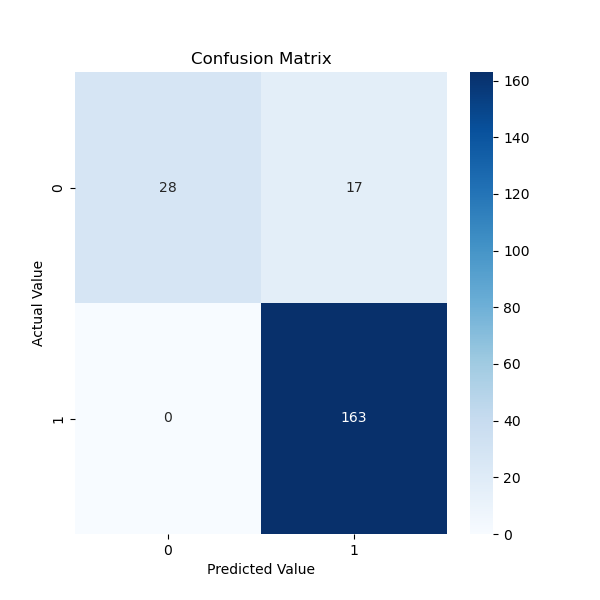
\includegraphics[width=0.6\textwidth]{confusion_matrix_Logistic_Regression.png}
  \caption{Confusion Matrix for the LR Model}
  \label{fig:lg_confusion_matrix}
\end{figure}
From these values, we calculate:

\begin{table}[h!]
\centering
\caption{Evaluation Metrics for the LR Model}
\label{tab:evaluation_metrics_LR_test}
\begin{tabular}{|l|c|}
\hline
\textbf{Metric} & \textbf{Value} \\
\hline
Accuracy       & 0.8942 \\
Precision      & 0.8925 \\
Recall         & 0.9881 \\
F1 Score       & 0.9379 \\
ROC AUC (Test) & 0.8708 \\
\hline
\end{tabular}
\end{table}

These metrics from Table \ref{tab:evaluation_metrics_LR_test} confirm that logistic regression did not just guess correctly by chance, but was able to learn meaningful patterns from the dataset.

A particularly interesting finding emerged when reducing the number of features: even with only the 10 most important features (instead of the original 100), the prediction performance remained nearly constant. This illustrates two key points:

Feature selection is highly effective for logistic regression. The model can focus on the essential influencing variables without unnecessary “feature noise” distorting the results.

The reduction minimizes the effect of the curse of dimensionality. In high dimensions, many data points lose their separability, especially in distance-based methods - although logistic regression is less sensitive to high dimensionality than methods like KNN or SVM. Nevertheless, it benefits from excluding irrelevant or highly correlated features.

The observation that model predictions remained nearly identical despite a massive reduction in feature number speaks to the robustness and generalization ability of logistic regression - at least under the given conditions.

\citep{hosmer2013logistic}

\subsection{K Nearest Neighbors}

To assess the performance of the KNN classifier, we analyzed the confusion matrix (Figure \ref{fig:confusion_matrix_KNN}) and computed key metrics.

\begin{figure}[h]
  \centering
  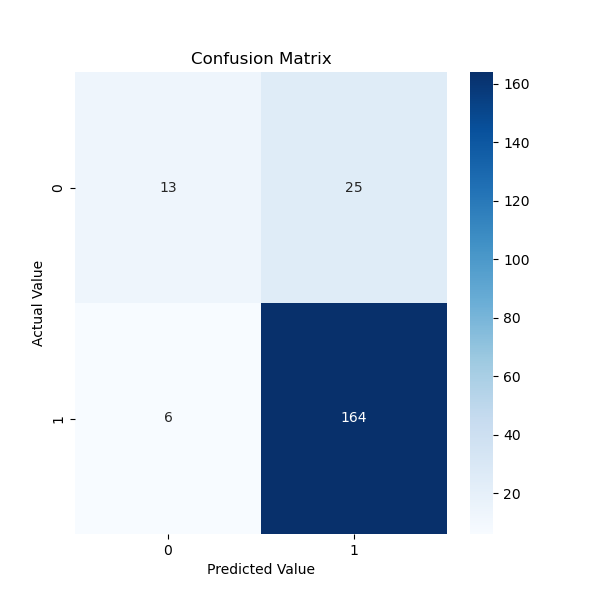
\includegraphics[width=0.6\textwidth]{confusion_matrix_KNN.png}
  \caption{Confusion Matrix for the KNN Model}
  \label{fig:confusion_matrix_KNN}
\end{figure}

From this, we calculate:

\begin{table}[h!]
\centering
\caption{Evaluation Metrics for the KNN Model}
\label{tab:evaluation_metrics_class1}
\begin{tabular}{|l|c|}
\hline
\textbf{Metric} & \textbf{Value} \\
\hline
Accuracy  & 0.8510 \\
Recall (Sensitivity) for Class 1 & 0.9821 \\
Precision for Class 1 & 0.8549 \\
F1 Score  & 0.9141 \\
ROC AUC   & 0.7771 \\
\hline
\end{tabular}
\end{table}

Table \ref{tab:evaluation_metrics_class1} shows that the model performs well at detecting positive cases (class 1), with a very high recall of 96.5\%. This makes it suitable for applications where missing a positive case is costly.
However, it misclassified 29 out of 40 negative cases (class 0), correctly identifying only 11, which shows a weakness in detecting negatives.
Despite a strong F1-score and precision, the ROC AUC of 0.709 indicates that KNN struggles to distinguish between classes overall.
KNN achieves high accuracy and excellent performance on positive cases, but it is not reliable for detecting negative cases. Its predictive power is skewed toward class 1, which is important to consider depending on the use case. \citep{ibm-knn}


\section{Discussion}

\subsection{Interpretation of Results}

Our analysis evaluated four classical machine learning models - Support Vector Machine (SVM), Logistic Regression (LR), Random Forest (RF), and k-Nearest Neighbors (kNN) - to predict Ceftriaxone resistance in \textit{Escherichia coli} using MALDI-TOF mass spectrometry data. Each model offered unique strengths and trade-offs, highlighting different potential use cases in clinical diagnostics.

The Support Vector Machine model emerged as the top overall performer, achieving the highest ROC AUC (0.9149), as well as strong precision (0.9408), recall (0.9464), and F1 score (0.9436). This balanced performance indicates that SVM is highly effective at discriminating between resistant and sensitive strains, making it well-suited for diagnostic decision support, where both sensitivity and specificity are important.

Logistic Regression also demonstrated excellent predictive capability, with a recall of 0.9881 and an F1 score of 0.9379. Its precision (0.8925) and ROC AUC (0.8708) were slightly lower than SVM, but still within clinically acceptable ranges. The model's simplicity and interpretability make it a practical choice in settings requiring transparent decision-making.

Random Forest achieved perfect recall (1.000), identifying all resistant cases in the test set. However, this high sensitivity came with a lower precision (0.8235) and ROC AUC (0.8242), indicating more false positives. This suggests RF may be best applied in preliminary screening, where missing resistant cases is more critical than minimizing false alarms.

The k-Nearest Neighbors model achieved a precision of 0.8549, a strong F1 score of 0.9141, and a recall of 0.9821 for the resistant class. However, it posted the lowest ROC AUC (0.7771) among all models, indicating reduced discriminative ability across both classes. This suggests that while kNN is highly effective at identifying resistant strains, it may struggle with accurate classification of sensitive cases, likely due to class imbalance and the high dimensionality of the feature space.


In summary, SVM provided the best balance across all evaluation metrics and stands out as the most promising candidate for predictive diagnostics in this context. Logistic Regression offers a strong, interpretable alternative, while Random Forest's perfect sensitivity makes it useful for conservative screening. kNN, despite strong precision, appears less suited due to its class imbalance sensitivity and lower discriminative power.


\subsection{Comparison to Previous Work}

Our findings align closely with Weis et al. (2022), who also demonstrated comparable performance (ROC AUC 0.85-0.93) using convolutional neural networks on MALDI-TOF spectra. Notably, our classical models (Logistic Regression and SVM) achieved similar predictive accuracy but with significantly reduced computational complexity and enhanced interpretability, valuable traits for clinical integration. Astudillo et al. (2024) further support our results, highlighting Random Forest and Logistic Regression's utility and effectiveness in rapid, accurate antibiotic resistance prediction using MALDI-TOF data.

\subsection{Limitations and Suggested Improvements}

This study has several limitations. Although we used class weighting to address the dataset's imbalance, advanced methods like SMOTE or generative models could enhance generalizability. The absence of annotated biological markers for spectral features restricts interpretability; future work should integrate genomic or proteomic analyses to associate spectral peaks with known resistance mechanisms explicitly. Additionally, our model evaluation utilized a random train-test split without institutional stratification, potentially limiting cross-institutional generalizability. Lastly, assessing only classical models limits exploration of potentially superior machine learning methods such as gradient boosting or neural network architectures.

\subsection{Conclusions and Future Outlook}

Future investigations should implement cross-institutional validation to evaluate robustness and clinical applicability thoroughly. Integrating model-agnostic interpretation methods like SHAP or LIME could clarify biological relevance and foster clinical acceptance. Broadening model comparisons to include advanced architectures like XGBoost or deep learning might further enhance predictive performance. Lastly, assessing practical clinical integration, including turnaround time, diagnostic accuracy, and patient outcomes, is paramount for translating these methods into routine diagnostic use.

Overall, our results affirm that classical machine learning models can effectively predict Ceftriaxone resistance in \textit{E. coli} from MALDI-TOF spectra, providing a promising foundation for future validation, interpretation, and clinical integration.



\bibliographystyle{plainnat}

\bibliography{bibliography}


\end{document}




%%				cd  /Users/user/Desktop/project/project/report 			pdflatex -shell-escape Report.tex

%%															bibtex report   
